\documentclass[../taasin.tex]{subfiles}
\graphicspath{{\subfix{../figures/}}}
\begin{document}
\label{appendix:snn}

%%%%%%%%%%%%%%%%%%%%%%%%%%%%%%%%%%%%%%%%%%%%%%%%%%%%%%%%%%%%%%%%%%%%%%

To implement a SNN, I used a python package built on top of PyTorch called snnTorch \cite{snnTorch}. The main way that SNNs differ from normal artificial neural networks (ANNs) is that the activation function only outputs either a 1 (a "spike") or a 0 and that inputs vary over time. Neurons maintain an internal voltage that increases when their inputs spike and decays in the absence of input. This allows SNNs to replace floating point multiplications with simple additions because the synapse weight is only multiplied by a 1 or a 0.

%********************************************************************%

\subsection{Circuit Model of a Spiking Neuron}

The fundamental unit of an SNN is the leaky integrate and fire (LIF) neuron. It can be represented as an RC circuit as show in figure \ref{fig:rc_circuit}.

\begin{figure}[h]
    \centering
    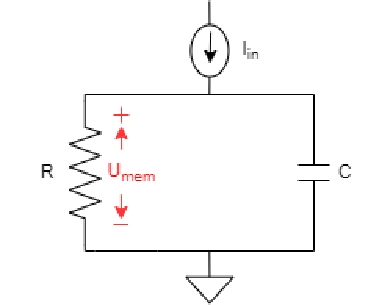
\includegraphics[width=0.5\textwidth]{figures/RC_neuron.pdf}
    \caption{The RC circuit representing a leaky integrate and fire neuron.}
    \label{fig:rc_circuit}
\end{figure}


From the circuit we can use Kirchoff's current law, and reach the equation below.

$$ I_{in}(t) = I_R + I_C $$

Now we want to derive equations for $ I_R $ and $ I_C $. We use Ohm's law, $ I = V/R $, for the resistor and the relationship $ Q = CU_{mem}(t) $ for the capacitor. V is the voltage across the resistor and Q is the charge on the capacitor.  

$$ I_R(t) = \frac{U_{mem}(t)}{R} $$

$$ I_C(t) = \frac{dQ}{dt} = C \frac{dU_{mem}(t)}{dt} $$

Now we place these definitions into our original equation and algebraically solve for $ \frac{dU_{mem}(t)}{dt} $.

$$ I_{in}(t) = \frac{U_{mem}(t)}{R} + C \frac{dU_{mem}(t)}{dt} $$
$$ RC \frac{dU_{mem}(t)}{dt} = -U_{mem}(t) + RI_{in}(t)$$

The units of the RHS are in voltage, while the term $\frac{dU_{mem}(t)}{dt}$ is voltage/time. Therefore the units of $RC$ must be in time, and we refer to this as the time constant $\tau$. This is a standard ordinary differential equation. We could solve it to get that $ U_{mem}(t) = U_0 e ^{\frac{-t}{\tau}} $, but this isn't useful in a discreet time neural network. Therefore, we use the definition of a derivative to get the following form.

$$ \tau \frac{dU(t)}{dt} = -U(t) + RI_{in}(t) $$
$$ \tau \frac{U(t + \Delta t) - U(t)}{\Delta t}  = -U(t) + RI_{in}(t) $$
$$ U(t + \Delta t) = U(t) + \frac{\Delta t}{\tau} (-U(t) + RI_{in}(t)) $$

% Insert graph of decaying membrane w/o input but increasing with input

With this equation we have what we want. A membrane potential that increases with input current and decays in the absence of any input. The equation still has a lot of hyperparameters, which would be very difficult to tune. The snnTorch package simplifies the equation in the following way.

$$ U(t + \Delta t) = (1 - \frac{\Delta t}{\tau}) U(t) + \frac{\Delta t}{\tau} R I_{in}(t)$$

Assuming $ I_{in}(t) = 0 $.

$$ U(t + \Delta t) = (1 - \frac{\Delta t}{\tau}) U(t) $$

We simplify the term $(1 - \frac{\Delta t}{\tau})$ to $\beta$, the decay rate. Note that $ \Delta t << \tau $ for reasonable accuracy. 

$$ U(t + \Delta t) = \beta U(t) $$

% skipped W derivation, not clear in tutorial
Because we want to work with discreet timesteps, we can assume $\Delta t = 1$. We also assume $R=1$ to reduce the number of hyperparameters. This brings us to the equation

$$ U(t+1) = \beta U(t) + W X(t+1) $$

$W$ is a learnable parameter that weights the input spikes $X$. With $S[t]$ as our spiking function, we add a term to reset the membrane voltage when this neuron outputs a spike. Our final equations are:

$$ U[t+1] = \underbrace{\beta U(t)}_{\text{decay}}
+ \underbrace{W X(t+1)}_{\text{input}}
- \underbrace{S(t)U_{thr}}_{\text{reset}} 
$$

$$
S[t] = \begin{cases} 
      1 & \text{if } U(t) > U_{thr} \\
      0 & \text{otherwise }
      \end{cases}
$$

%********************************************************************%

\subsection{Loop Unroll}

From a computational graph perspective, SNNs are very similar to recurrent neural networks (RNNs). This also shows how backpropagation through time (BPTT) can be used to calculate the gradients.

\begin{figure}[h]
    \centering
    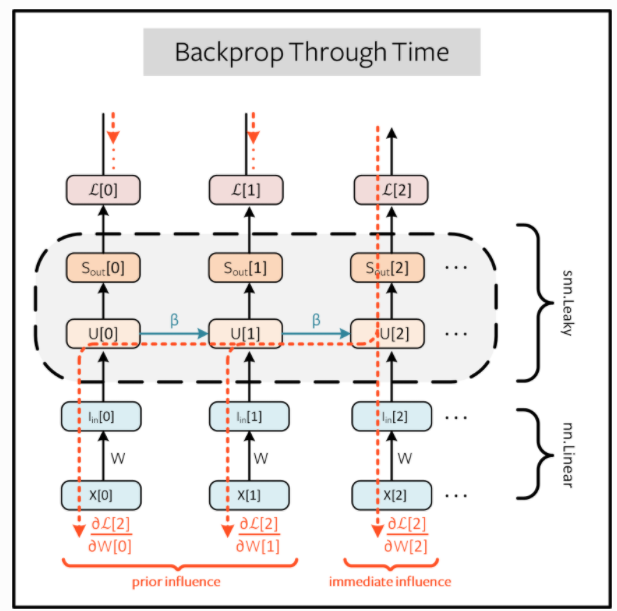
\includegraphics[width=0.4\textwidth]{figures/snnTorch_bptt.png}
    \caption{Computation graph for a SNN, similar to a RNN. Taken from \cite{snnTorch}.}
    \label{fig:snn_loop_unroll}
\end{figure}

%********************************************************************%

\subsection{Neuron Parameters}

There are a few choices that we have in the types of neurons that we select to use.

We treat $\beta$ as a hyperparameter, although it can also be trained in different ways. Tuning it on a per-layer or individual neuron basis with backpropagation may be interesting for future work.

The threshold voltage for each neuron is initialized to 1 but is a trainable parameter during backpropagation.

We have two options regarding what to do when the membrane voltage is larger than the threshold voltage. We can either reset the membrane voltage to zero or subtract the threshold voltage from the current membrane voltage. We refer to these techniques as "reset" and "subtract," respectively. With the subtract method, the neuron will have a non-zero membrane voltage if it was heavily excited. These methods simulate how a real neuron is inhibited from firing for a short period of time after it spikes. Resetting results in sparser spiking and potential energy savings, but is also more difficult to learn with. We use subtraction in our neurons.

% WTA
Inhibition is another interesting option. In real neurons, sometimes the activation of one neuron can inhibit other neurons from firing. Our more traditional architecture would have very sparse spiking with this type of learning enabled, so it was not used. However, spiking RNNs may benefit from this feature.

Neurons have a distinction between what is known as first and second order. A second order neuron accounts for the fact that when a presynaptic neuron fires, it takes time for the signal to reach the current neuron. This is accounted for by adding a second hyperparameter $\alpha$. These models are more complex to train and resulted in higher loss values, so our work uses first order spiking neurons.

%%%%%%%%%%%%%%%%%%%%%%%%%%%%%%%%%%%%%%%%%%%%%%%%%%%%%%%%%%%%%%%%%%%%%%

\end{document}